%======================================================================
\NEWSEC
%======================================================================

\subsection{\ssInstallEnzop}

%----------------------------------------------------------------------
\begin{frame}[fragile,label=ss-install-enzop] 
\secframetitle{\ssInstallEnzop}
\framesubtitle{Enzo-P source code: \url{https://bitbucket.org/cello-project}}
\footnotesize \enzopcello\ source is available from \textcolor{green!50!black}{\url{https://bitbucket.org/cello-project}}
\begin{center}
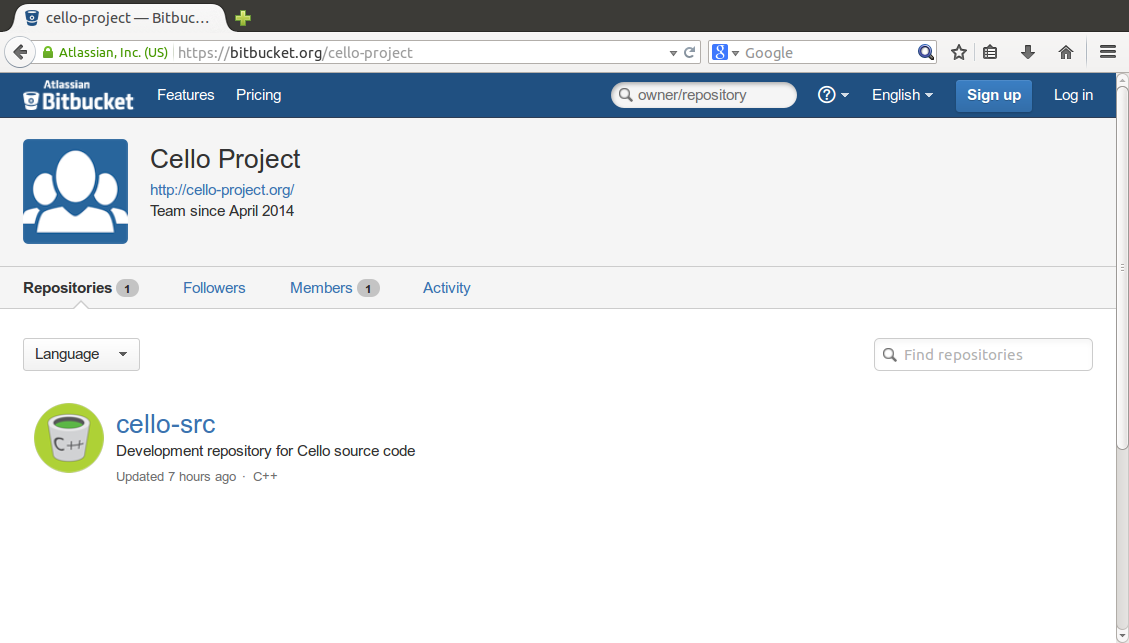
\includegraphics[width=4.00in]{cello-download.png}
\end{center}
\end{frame}
\setbeamercolor{monitor-2.png}{bg=RGB{43,43,51}}

%----------------------------------------------------------------------
\begin{frame}[fragile] 
\secframetitle{\ssInstallEnzop}
\framesubtitle{Downloading Enzo-P/Cello}
\footnotesize
\begin{semiverbatim}
\prompt\redcode{ mkdir \url{~}/Cello}\cursor{1}
\uncover<2->{\prompt\redcode{ cd \url{~}/Cello}\cursor{2}}
\uncover<3->{\prompt\redcode{ hg clone https://bitbucket.org/cello-project/cello-src}\cursor{3}}
\uncover<4->{destination directory: cello-src}
\uncover<4->{applying clone bundle from https://api.media.atlassian.com/\ldots}
\uncover<4->{adding changesets}
\uncover<4->{adding manifests}
\uncover<4->{adding file changes}
\uncover<4->{added 4024 changesets with 26817 changes to 4774 files (+2 heads)}
\uncover<4->{\ldots}
\uncover<4->{getting input/method_cosmology-8.in}
\uncover<4->{getting input/method_cosmology.incupdating to branch default}
\uncover<4->{resolving manifests}
\uncover<4->{1056 files updated, 0 files merged, 0 files removed, 0 files unresolved}
\end{semiverbatim}
\end{frame}

